\section{Specifica dei test}

\begin{itemize}
    \item \textbf{Test di unità:} vengono effettuati per verificare che il comportamento di ogni singolo componente sia corretto;
    \item \textbf{Test di integrazione:} vengono effettuati per verificare che il comportamento dei componenti messi in relazione sia corretto;
    \item \textbf{Test di sistema:} vengono effettuati per assicurare che i requisiti identificati nel documento Analisi dei Requisiti v1.0.0 siano rispettati.
    \item \textbf{Test di accettazione:} vengono effettuati insieme al proponente durante la fase di collaudo.
\end{itemize}
\section{Test di unità}
I test di unità verranno stabiliti nel periodo di Progettazione di dettaglio e codifica.

\section{Test di integrazione}
I test di integrazione verranno stabiliti nel periodo di Progettazione di dettaglio e codifica.

\section{Test di sistema}
\renewcommand{\arraystretch}{1.5}
\rowcolors{2}{gray!25}{white}
\begin{longtable}{ m{0.15\textwidth}<{\centering}  m{0.5\textwidth}<{\centering}  m{0.25\textwidth}<{\centering} }
	\rowcolor{darkblue}
	\textcolor{white}{\textbf{Test}} &\textcolor{white}{\textbf{Descrizione}} & \textcolor{white}{\textbf{Implementazione}} \\ 

	TS	R1FW1 & Si verifica che l'utente riesca ad inserire correttamente i propri dati personali per effettuare la registrazione & \Ni \\
	TSR1FW2 & Si verifica che l'utente riesca ad inserire correttamente i propri dati personali per effettuare il login & \Ni \\
	TSR1FW3 & Si verifica che l'utente riesca a recuperare la password di accesso, nel caso l'avesse dimenticata & \Ni \\
	TSR1FE1 & Si verifica che all'utente venga mostrato un errore nel caso non venga inserito correttamente il nome in fase di registrazione & \Ni \\
	TSR1FE2 & Si verifica che all'utente venga mostrato un errore nel caso non venga inserito correttamente il cognome in fase di registrazione & \Ni \\
	TSR1FE3 & Si verifica che all'utente venga mostrato un errore nel caso non venga inserito correttamente l'indirizzo e-mail in fase di registrazione & \Ni \\
	TSR1FE4 & Si verifica che all'utente venga mostrato un errore nel caso non venga inserita correttamente la password in fase di registrazione & \Ni \\
	TSR1FE5 & Si verifica che all'utente venga mostrato un errore nel caso non venga inserito correttamente l'indirizzo e-mail in fase di login & \Ni \\
	TSR1FE6 & Si verifica che all'utente venga mostrato un errore nel caso non venga inserita correttamente la password in fase di login & \Ni \\
	TSR1FE7 & Si verifica che all'utente venga mostrato un errore nel caso non venga inserita correttamente la password in fase di recupero password & \Ni \\
	TSR1FW4 & Si verifica che un utente autenticato possa accedere alla sua area personale & \Ni \\
	TSR2FW4.1 & Si verifica che l'utente autenticato riesca a collegare correttamente il proprio profilo Instagram & \Ni \\
	TSR2FE8 & Si verifica che all'utente autenticato venga mostrato un messaggio d'errore nel caso il collegamento con il profilo Instagram non vada a buon fine & \Ni \\
	TSR2FW4.2 & Si verifica che l'utente autenticato riesca a collegare correttamente il proprio profilo TikTok & \Ni \\
	TSR2FE9 & Si verifica che all'utente autenticato venga mostrato un messaggio d'errore nel caso il collegamento con il profilo TikTok non vada a buon fine & \Ni \\
	TSR3FW4.3 & Si verifica che l'utente autenticato riesca a modificare la password con cui accede al sistema & \Ni \\
	TSR3FE15 & Si verifica che all'utente autenticato venga mostrato un errore nel caso non venga inserita una password valida in fase di modifica & \Ni \\
	TSR1FW5 & Si verifica che l'utente autenticato possa suggerire dei profili social da cui fare il crawling dei dati & \Ni \\
	TSR2FE10 & Si verifica che all'utente autenticato venga mostrato un errore nel caso suggerisca un profilo social inesistente & \Ni \\
	TSR2FE11 & Si verifica che all'utente autenticato venga mostrato un errore nel caso suggerisca un profilo social privato & \Ni \\
	TSR2FE12 & Si verifica che all'utente autenticato venga mostrato un errore nel caso suggerisca un profilo social già presente a sistema & \Ni \\
	TSR1FW7 & Si verifica che l'utente riesca a visualizzare la classifica con i locali presenti nel database & \Ni \\
	TSR1FW8 & Si verifica che l'utente riesca a filtrare la classifica & \Ni \\
	TSR2FE13 & Si verifica che all'utente venga mostrato un errore nel caso non ci sia alcun risultato compatibile con i filtri applicati & \Ni \\
	TSR1FW8.1 & Si verifica che l'utente riesca a filtrare la classifica dei locali presenti nel database in base alla zona & \Ni \\
	TSR2FW8.2 & Si verifica che l'utente riesca a filtrare la classifica dei locali presenti nel database per giorno ed orario di apertura & \Ni \\
	TSR2FW8.3 & Si verifica che l'utente riesca a filtrare la classifica dei locali presenti nel database in base al tipo di cucina & \Ni \\
	TSR2FW8.4 & Si verifica che l'utente riesca a filtrare la classifica dei locali presenti nel database per fascia di prezzo & \Ni \\
	TSR1FW8.5 & Si verifica che l'utente riesca a filtrare la classifica dei locali presenti nel database in base al punteggio & \Ni \\
	TSR3FW9 & Si verifica che l'utente riesca a modificare l'ordinamento di visualizzazione della classifica & \Ni \\
	TSR3FW9.1 & Si verifica che l'utente riesca a visualizzare i risultati della classifica impostando il peso dei social & \Ni \\
	TSR3FW9.2 & Si verifica che l'utente riesca a modificare i risultati della classifica impostando il peso dei tipi di contenuto & \Ni \\
	TSR1FW10 & Si verifica che l'utente riesca a cercare un locale presente nel database tramite il suo nome & \Ni \\
	TSR2FE14 & Si verifica che all'utente venga mostrato un errore nel caso il locale cercato non sia presente nel sistema & \Ni \\
	TSR1FW11 & Si verifica che l'utente riesca a visualizzare le informazioni di un locale presente nel sistema & \Ni \\
	TSR2FW12 & Si verifica che l'utente riesca ad aggiungere un locale nella lista dei preferiti & \Ni \\
	TSR2FW13 & Si verifica che l'utente riesca ad rimuovere un locale dalla lista dei preferiti & \Ni \\
	TSR3F1 & Si verifica che l'utente riesca a suggerire delle modifiche da apportare relative alle informazioni di un locale & \Ni \\
	
    \caption{Test di sistema}
\end{longtable}	

\subsubsection{Test di Sistema - Tracciamento dei requisiti}


\rowcolors{2}{gray!25}{white}
\renewcommand{\arraystretch}{1.5}
\begin{longtable}{ m{0.15\textwidth}<{\centering}  m{0.3\textwidth}<{\centering} }
	\rowcolor{darkblue}
	\textcolor{white}{\textbf{ID Test}} &\textcolor{white}{\textbf{ID Requisito}}\\ 
	 
	TS	R1FW1 & R1FW1 \\
	TSR1FW2 &  R1FW2 \\
	TSR1FW3 & R1FW3 \\
	TSR1FE1 & R1FE1 \\
	TSR1FE2 & R1FE2 \\
	TSR1FE3 & R1FE3 \\
	TSR1FE4 & R1FE4 \\
	TSR1FE5 & R1FE5 \\
	TSR1FE6 & R1FE6 \\
	TSR1FE7 & R1FE7 \\
	TSR1FW4 & R1FW4 \\
	TSR2FW4.1 & R2FW4.1 \\
	TSR2FE8 & R2FE8 \\
	TSR2FW4.2 & R2FW4.2 \\
	TSR2FE9 & R2FE9 \\
	TSR3FW4.3 & R3FW4.3\\
	TSR3FE15 & R3FE15 \\
	TSR1FW5 & R1FW5 \\
	TSR2FE10 & R2FE10 \\	 
	TSR2FE11 & R2FE11 \\
	TSR2FE12 & R2FE12 \\
	TSR1FW7 & R1FW7 \\
	TSR1FW8 & R1FW8 \\
	TSR2FE13 & R2FE13 \\
	TSR1FW8.1 & R1FW8.1 \\
	TSR2FW8.2 & R2FW8.2 \\
	TSR2FW8.3 & R2FW8.3 \\
	TSR2FW8.4 & R2FW8.4 \\
	TSR1FW8.5 & R1FW8.5 \\
	TSR3FW9 & R3FW9 \\
	TSR3FW9.1 & R3FW9.1 \\
	TSR3FW9.2 & R3FW9.2 \\
	TSR1FW10 & R1FW10 \\
	TSR2FE14 & R2FE14  \\
	TSR1FW11 & R1FW11 \\
	TSR2FW12 & R2FW12 \\
	TSR2FW13 & R2FW13 \\
	TSR3F1 & R3F1 \\

\caption{Tracciamento Test di Sistema - Requisiti}
\end{longtable}


\section{Test di accettazione}
I test di accettazione verranno stabiliti nel periodo di Progettazione di dettaglio e codifica.

\section{Resoconto attività di verifica}

\subsection{Periodo di Analisi}
In questo periodo vengono calcolate le metriche MPC01, MPC02, MPC03, MPC04, MPC05, MPC06, MPC07 e MQP01. Le restanti metriche non vengono calcolate dato che sono relative alla codifica.

\subsubsection{MPC01 - SPICE}
Ogni sigla presente in questa sezione fa riferimento a quanto descritto all'interno del documento NormeDiProgetto-v1.0.0 §A


TODO:Mettere una breve descrizione dei risultati e scrivere i risultati + istogramma alla fine 
\begin{table}[H]
    \rowcolors{2}{gray!25}{white}
    \rowcolors{2}{gray!25}{white}
        \renewcommand{\arraystretch}{1.5}
        \begin{tabular}{ m{0.15\textwidth}<{\centering}  m{0.055\textwidth}<{\centering} m{0.055\textwidth}<{\centering} m{0.055\textwidth}<{\centering} m{0.055\textwidth}<{\centering} m{0.055\textwidth}<{\centering} m{0.055\textwidth}<{\centering} m{0.055\textwidth}<{\centering} m{0.055\textwidth}<{\centering} m{0.055\textwidth}<{\centering} m{0.08\textwidth}<{\centering}}
	\rowcolor{darkblue}
	\textcolor{white}{\textbf{Processo}} &\textcolor{white}{\textbf{1.1}} &\textcolor{white}{\textbf{2.1}} &\textcolor{white}{\textbf{2.2}} &\textcolor{white}{\textbf{3.1}} &\textcolor{white}{\textbf{3.2}} &\textcolor{white}{\textbf{4.1}} &\textcolor{white}{\textbf{4.2}} &\textcolor{white}{\textbf{5.1}} &\textcolor{white}{\textbf{5.2}} &\textcolor{white}{\textbf{Livello}}\\ 

    Fornitura & F & F & F & N & N & N & N & N & N & 2 \\
    Sviluppo & F & F & F & N & N & N & N & N & N & 2 \\
    Documentazione & F & F & F & N & N & N & N & N & N & 2 \\
    Gestione della configurazione & F & F & F & N & N & N & N & N & N & 2 \\
    Gestione della qualità & F & F & F & N & N & N & N & N & N & 2 \\
    Verifica & F & F & F & N & N & N & N & N & N & 2 \\
    Validazione & F & F & F & N & N & N & N & N & N & 2 \\
    Gestione di processo & F & F & F & N & N & N & N & N & N & 2 \\
    Formazione dei membri del team & F & F & F & N & N & N & N & N & N & 2 \\
    
    \end{tabular}
\caption{Analisi: MPC01 - SPICE}
\end{table}

\subsubsection{MPC02 - BCWS}
\begin{figure}[H]
    \centering
    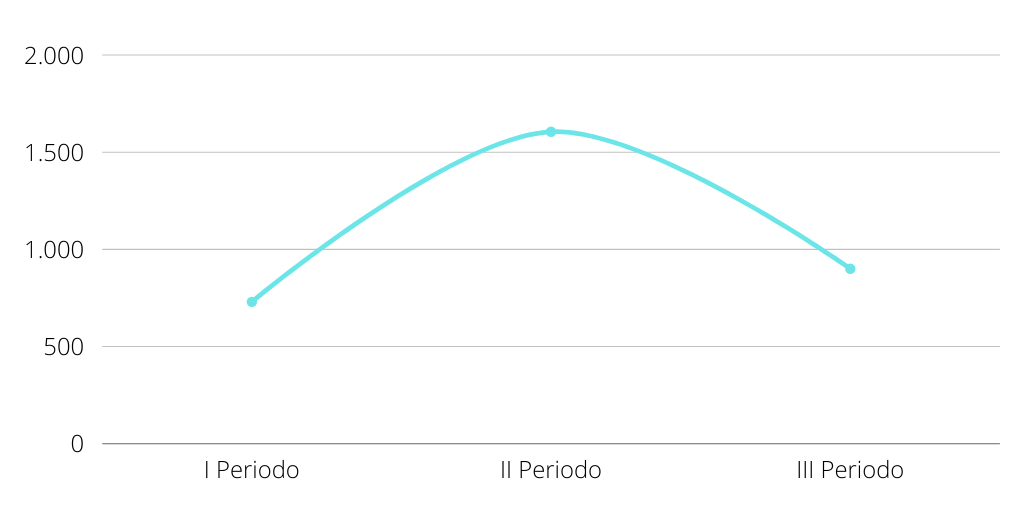
\includegraphics[scale=0.50]{Sezioni/images/analisi-bcws.png}
    \caption{Analisi: MPC02 - BCWS}
\end{figure}

\subsubsection{MPC03 - ACWP}
\begin{figure}[H]
    \centering
    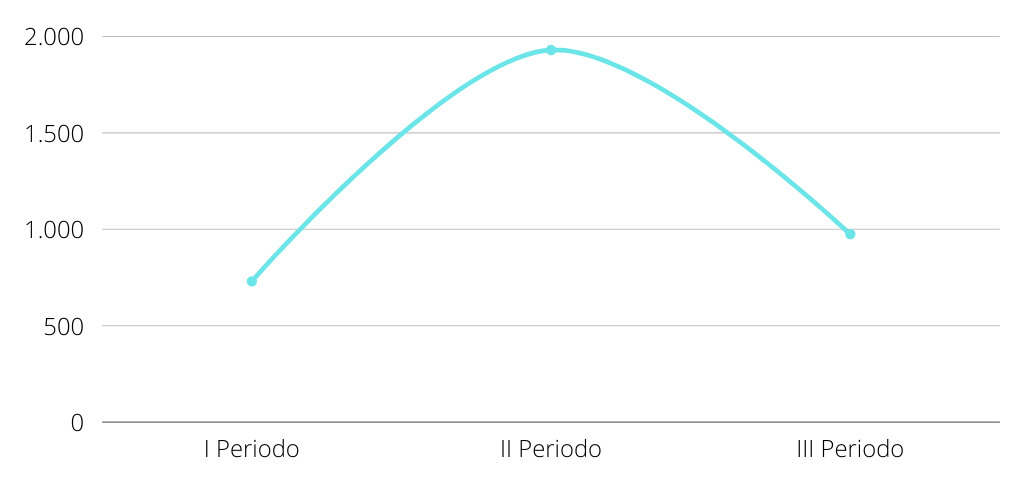
\includegraphics[scale=0.50]{Sezioni/images/analisi-acwp.png}
    \caption{Analisi: MPC02 - ACWP}
\end{figure}

\subsubsection{MPC04 - BCWP}
Nel primo periodo il BCWP è inferiore al BCWS a causa di un errore nell'analisi dei requisiti, il costo è stato recuperato nel periodo successivo.
\begin{figure}[H]
    \centering
    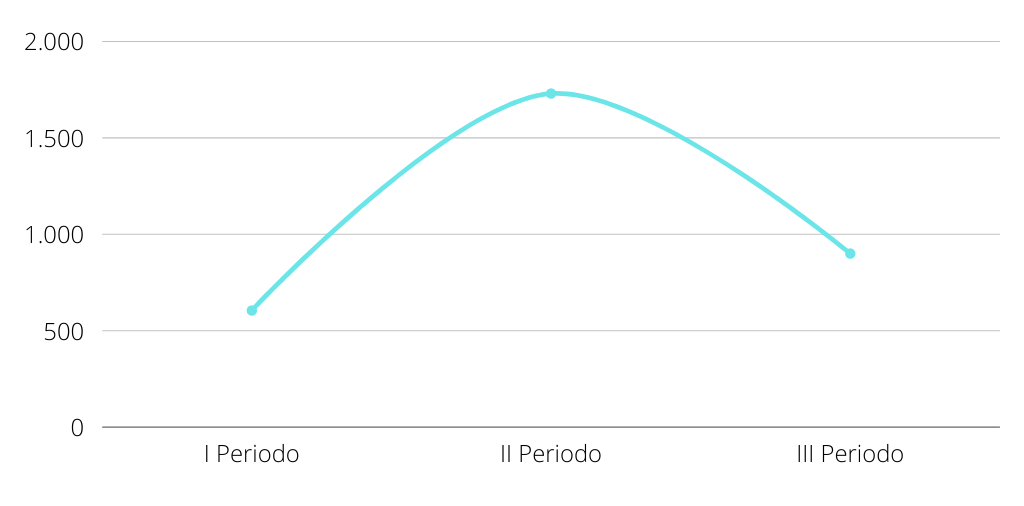
\includegraphics[scale=0.50]{Sezioni/images/analisi-BCWP.png}
    \caption{Analisi: MPC04 - BCWP}
\end{figure}

\subsubsection{MPC05 - Schedule variance}
\begin{figure}[H]
    \centering
    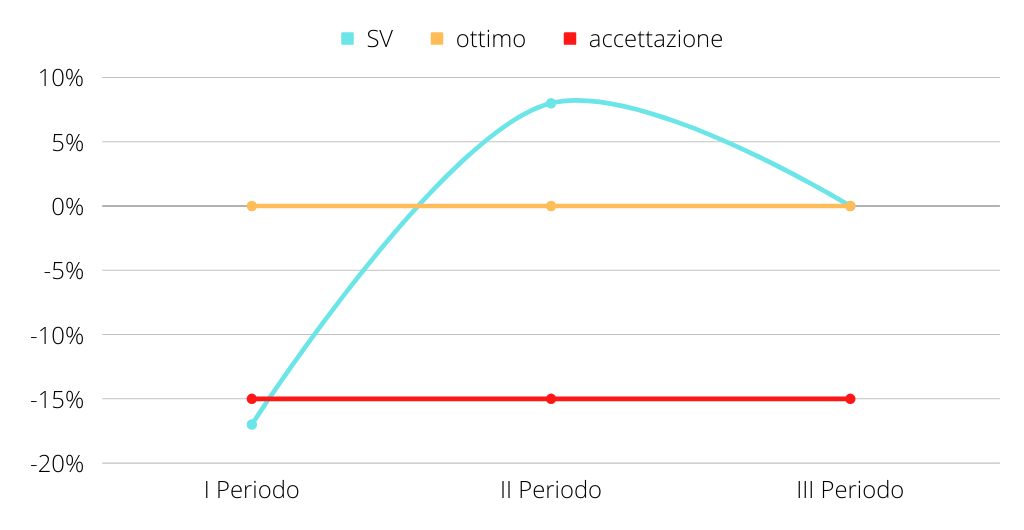
\includegraphics[scale=0.50]{Sezioni/images/analisi-SV.png}
    \caption{Analisi: MPC05 - SV}
\end{figure}

\subsubsection{MPC06 - Budget variance}
\begin{figure}[H]
    \centering
    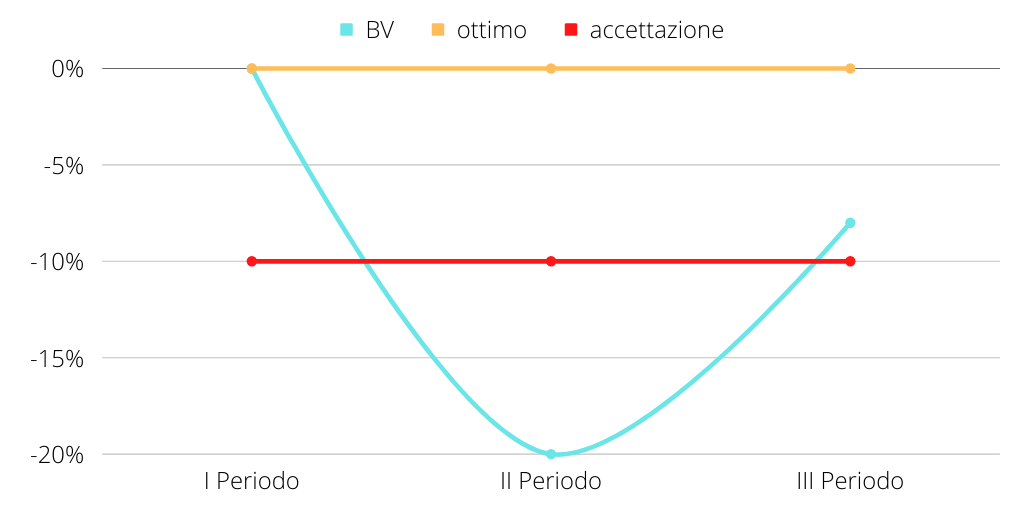
\includegraphics[scale=0.50]{Sezioni/images/analisi-BV.png}
    \caption{Analisi: MPC06 - BV}
\end{figure}

\subsubsection{MQP01 - Indice di Gulpease}
É stato calcolato l'indice di Gulpease di ogni documento redatto escludendo intestazione, registro delle modifiche e dati presenti nelle tabelle al fine di evitare risultati inesatti.
\begin{table}[H]
    \rowcolors{2}{gray!25}{white}
    \rowcolors{2}{gray!25}{white}
        \renewcommand{\arraystretch}{1.5}
        \begin{tabular}{m{0.4\textwidth}<{\centering}  m{0.25\textwidth}<{\centering}  m{0.25\textwidth}<{\centering} }
            \rowcolor{darkblue}
            \textcolor{white}{\textbf{Documento}}& \textcolor{white}{\textbf{Valore}} & \textcolor{white}{\textbf{Esito}}\\ 
            
			Norme di Progetto v0.x.0 &
            xxx &
            Superato \\

            Piano di Progetto v0.x.0 &
            xxx &
            Superato \\

            Piano di Qualifica v0.x.0 &
            xxx &
            Superato \\

            Analisi dei Requisiti v0.x.0 &
            xxx &
            Superato \\
            
            Glossario v0.x.0 &
            xxx &
            Superato \\

            VerbaleInterno-2021.11.22&
            75 &
            Superato \\

            VerbaleInterno-2021.11.29&
            75 &
            Superato \\
            
            VerbaleInterno-2021.12.06&
            64 &
            Superato \\
            
            VerbaleInterno-2021.12.13&
            61 &
            Superato \\
            
            VerbaleInterno-2021.12.20&
            77 &
            Superato \\
            
            VerbaleInterno-2021.12.29&
            76 &
            Superato \\
            
            VerbaleInterno-2022.01.03&
            77 &
            Superato \\
            
            VerbaleInterno-2022.01.07&
            66 &
            Superato \\
            
            VerbaleInterno-2022.01.09&
            88 &
            Superato \\
            
            VerbaleInterno-2022.01.13&
            76 &
            Superato \\
            
            VerbaleInterno-2022.01.20&
            65 &
            Superato \\

            Verbale Esterno-2021.12.22&
            75&
            Superato \\
            
    
    \end{tabular}
    \caption{Periodo di analisi MQP01}

	TODO:da mettere istogramma generale
	TODO: per i documenti che non sono verbali c'è da calcolare gulpease per il periodo fino al 22 gennaio e fare grafico cartesiano di ognuno
\end{table}

\subsection{Periodo di produzione del Proof of Concept}

\subsubsection{MPC01 - SPICE}
Ogni sigla presente in questa sezione fa riferimento a quanto descritto all'interno del documento NormeDiProgetto-v1.0.0 §A

TODO:Mettere una breve descrizione dei risultati e scrivere i risultati + istogramma alla fine 

\begin{table}[H]
    \rowcolors{2}{gray!25}{white}
    \rowcolors{2}{gray!25}{white}
        \renewcommand{\arraystretch}{1.5}
        \begin{tabular}{ m{0.15\textwidth}<{\centering}  m{0.055\textwidth}<{\centering} m{0.055\textwidth}<{\centering} m{0.055\textwidth}<{\centering} m{0.055\textwidth}<{\centering} m{0.055\textwidth}<{\centering} m{0.055\textwidth}<{\centering} m{0.055\textwidth}<{\centering} m{0.055\textwidth}<{\centering} m{0.055\textwidth}<{\centering} m{0.08\textwidth}<{\centering}}
	\rowcolor{darkblue}
	\textcolor{white}{\textbf{Processo}} &\textcolor{white}{\textbf{1.1}} &\textcolor{white}{\textbf{2.1}} &\textcolor{white}{\textbf{2.2}} &\textcolor{white}{\textbf{3.1}} &\textcolor{white}{\textbf{3.2}} &\textcolor{white}{\textbf{4.1}} &\textcolor{white}{\textbf{4.2}} &\textcolor{white}{\textbf{5.1}} &\textcolor{white}{\textbf{5.2}} &\textcolor{white}{\textbf{Livello}}\\ 

    Fornitura & F & F & F & N & N & N & N & N & N & 2 \\
    Sviluppo & F & F & F & N & N & N & N & N & N & 2 \\
    Documentazione & F & F & F & N & N & N & N & N & N & 2 \\
    Gestione della configurazione & F & F & F & N & N & N & N & N & N & 2 \\
    Gestione della qualità & F & F & F & N & N & N & N & N & N & 2 \\
    Verifica & F & F & F & N & N & N & N & N & N & 2 \\
    Validazione & F & F & F & N & N & N & N & N & N & 2 \\
    Gestione di processo & F & F & F & N & N & N & N & N & N & 2 \\
    Formazione dei membri del team & F & F & F & N & N & N & N & N & N & 2 \\
    Progettazione & F & F & F & N & N & N & N & N & N & 2 \\
    Codifica & F & F & F & N & N & N & N & N & N & 2 \\
        \end{tabular}
\caption{Produzione del Proof of Concept: MPC01 - SPICE}
\end{table}
\subsubsection{MPC02 - BCWS}
\begin{figure}[H]
    \centering
    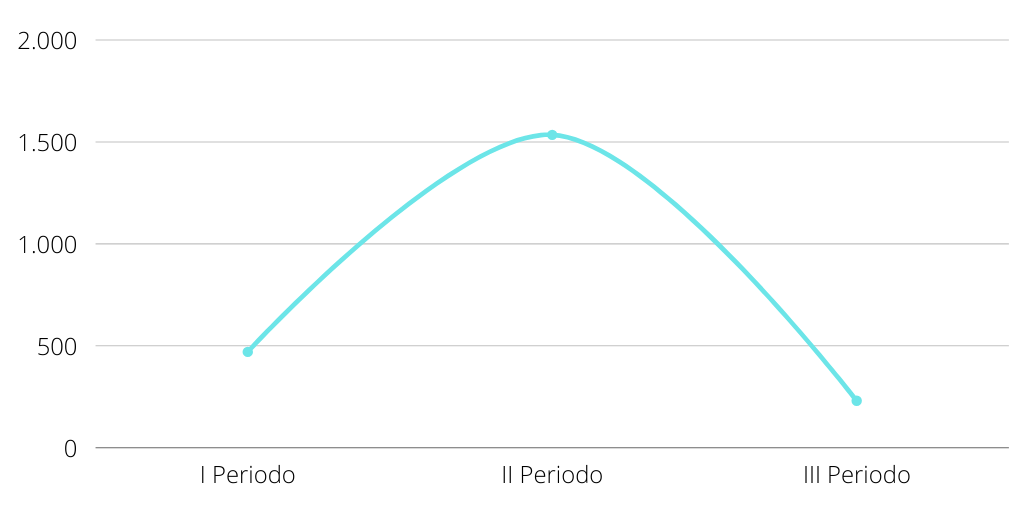
\includegraphics[scale=0.50]{Sezioni/images/poc-bcws.png}
    \caption{Produzione del Proof of Concept: MPC02 - BCWS}
\end{figure}

\subsubsection{MPC03 - ACWP}
\begin{figure}[H]
    \centering
    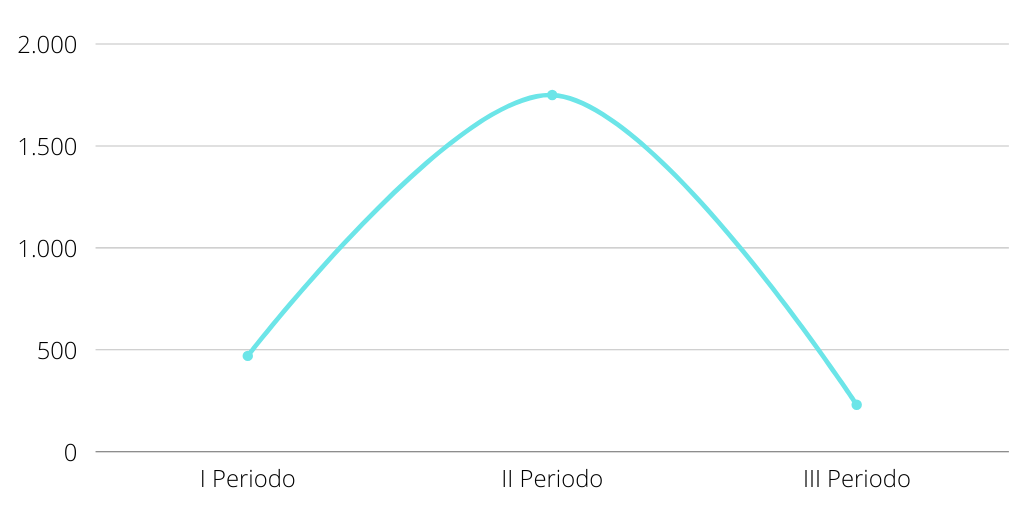
\includegraphics[scale=0.50]{Sezioni/images/poc-acwp.png}
    \caption{Produzione del Proof of Concept: MPC03 - ACWP}
\end{figure}

\subsubsection{MPC04 - BCWP}
Nel primo periodo il BCWP è inferiore al BCWS a causa di un incomprensione per la realizzazione del Proof of Concept, il costo in questione è stato recuperato nel periodo successivo.
\begin{figure}[H]
    \centering
    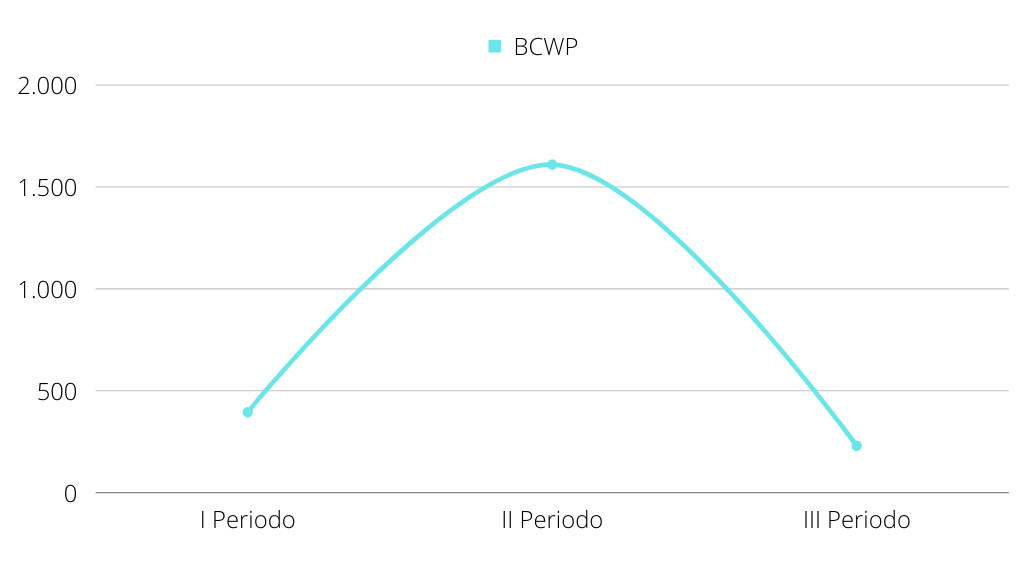
\includegraphics[scale=0.50]{Sezioni/images/poc-BCWP.png}
    \caption{Produzione del Proof of Concept: MPC04 - BCWP}
\end{figure}

\subsubsection{MPC05 - Schedule variance}
\begin{figure}[H]
    \centering
    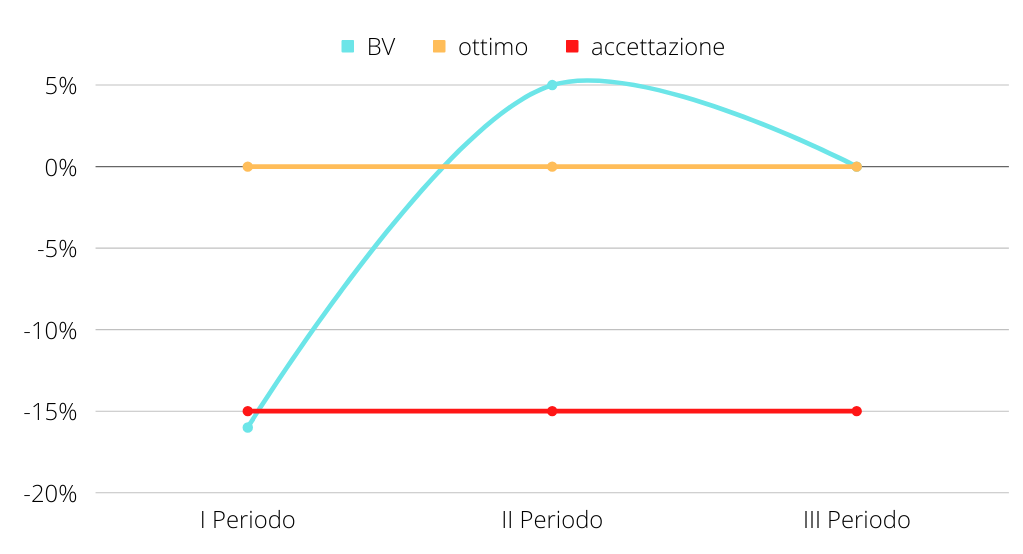
\includegraphics[scale=0.50]{Sezioni/images/poc-SV.png}
    \caption{Produzione del Proof of Concept: MPC05 - SV}
\end{figure}

\subsubsection{MPC06 - Budget variance}
\begin{figure}[H]
    \centering
    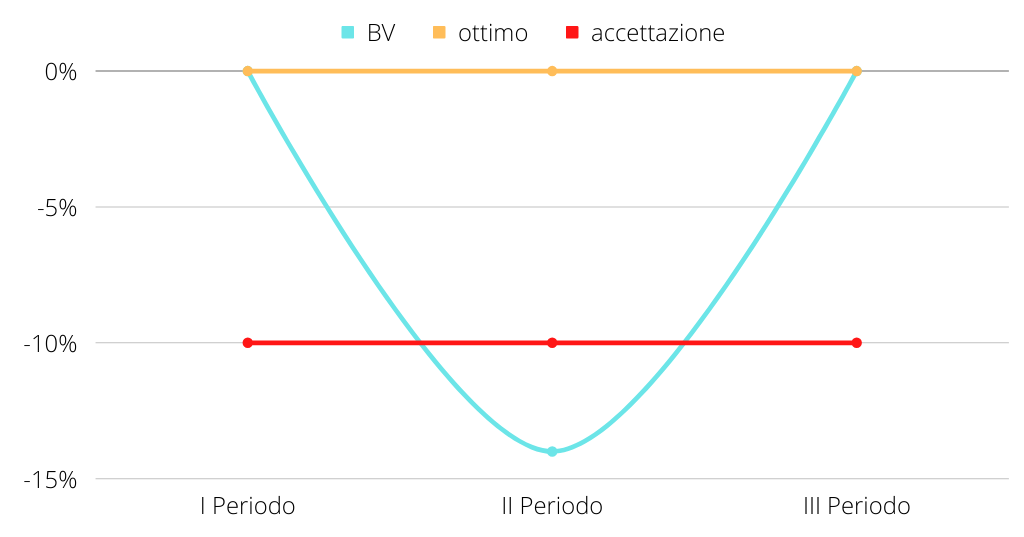
\includegraphics[scale=0.50]{Sezioni/images/poc-BV.png}
    \caption{Produzione del Proof of Concept: MPC06 - BV}
\end{figure}

\subsubsection{MQP01 - Indice di Gulpease}
\begin{table}[H]
    \rowcolors{2}{gray!25}{white}
    \rowcolors{2}{gray!25}{white}
        \renewcommand{\arraystretch}{1.5}
        \begin{tabular}{m{0.4\textwidth}<{\centering}  m{0.25\textwidth}<{\centering}  m{0.25\textwidth}<{\centering} }
            \rowcolor{darkblue}
            \textcolor{white}{\textbf{Documento}}& \textcolor{white}{\textbf{Valore}} & \textcolor{white}{\textbf{Esito}}\\ 

            Norme di Progetto v1.0.0 &
            xxx &
            Superato \\

            Piano di Progetto v1.0.0 &
            xxx &
            Superato \\

            Piano di Qualifica v1.0.0 &
            xxx &
            Superato \\

            Analisi dei Requisiti v1.0.0 &
            xxx &
            Superato \\
            
            Glossario v1.0.0 &
            xxx &
            Superato \\

            VerbaleInterno-2022.01.27&
            60 &
            Superato \\
            
            VerbaleInterno-2022.02.03&
            60 &
            Superato \\

            Verbale Esterno-2022.01.26&
            57&
            Superato \\

            Verbale Esterno-2022-02-08&
            61&
            Superato \\
    \end{tabular}
    \caption{Periodo di produzione del Proof of Concept - MQP01}\
	TODO:da mettere istogramma generale
	TODO: per i documenti che non sono verbali c'è da calcolare gulpease fino a 1.0.0 e fare grafico cartesiano di ognuno
\end{table}